% !TEX root = main.tex
\section{実験方法}

本実験では,段階的にWebデータベースを構築するため,複数のステップに分けて作業を行った.ここでは,まず最初に行ったXAMPPのインストールおよび動作確認について記述する.

\subsection*{環境}
\begin{itemize}
  \item OS:Ubuntu 22.04 LTS
\end{itemize}

\subsection*{実験Ⅰ:XAMPPのインストールと起動確認}

XAMPPは,Apache Webサーバ,MySQL(MariaDB),PHP,Perl などを一括でインストール・管理できるパッケージである.本実験では,XAMPPをインストールしてApacheの起動確認を行った.

\vspace{1zh}
\noindent 手順は以下の通りである.

\begin{enumerate}
  \item 以下の公式サイトより,XAMPPのLinux版インストーラをダウンロードする.
        \url{https://www.apachefriends.org/jp/index.html}

  \item ターミナルでダウンロードディレクトリに移動する.
        \begin{lstlisting}[language=bash]
cd ~/Downloads/
\end{lstlisting}

  \item インストーラに実行権限を与える.
        \begin{lstlisting}[language=bash]
sudo chmod 755 xampp-linux-x64-8.0.10-0-installer.run
\end{lstlisting}

  \item インストーラを実行する.
        \begin{lstlisting}[language=bash]
sudo ./xampp-linux-x64-8.0.10-0-installer.run
\end{lstlisting}

  \item GUIベースのマネージャを起動する.
        \begin{lstlisting}[language=bash]
sudo /opt/lampp/manager-linux-x64.run
\end{lstlisting}

  \item LAMP環境を起動する.
        \begin{lstlisting}[language=bash]
sudo /opt/lampp/lampp start
\end{lstlisting}

  \item ブラウザで \texttt{http://localhost/} を開き,「XAMPPへようこそ」と表示されればApacheの動作確認は完了である.

  \item 確認後,LAMP環境を停止する.
        \begin{lstlisting}[language=bash]
sudo /opt/lampp/lampp stop
\end{lstlisting}


\end{enumerate}

この操作により,Webサーバの動作環境が整い,今後のWebデータベース構築に必要な基盤が準備された.

\begin{figure}[htbp]
  \centering
  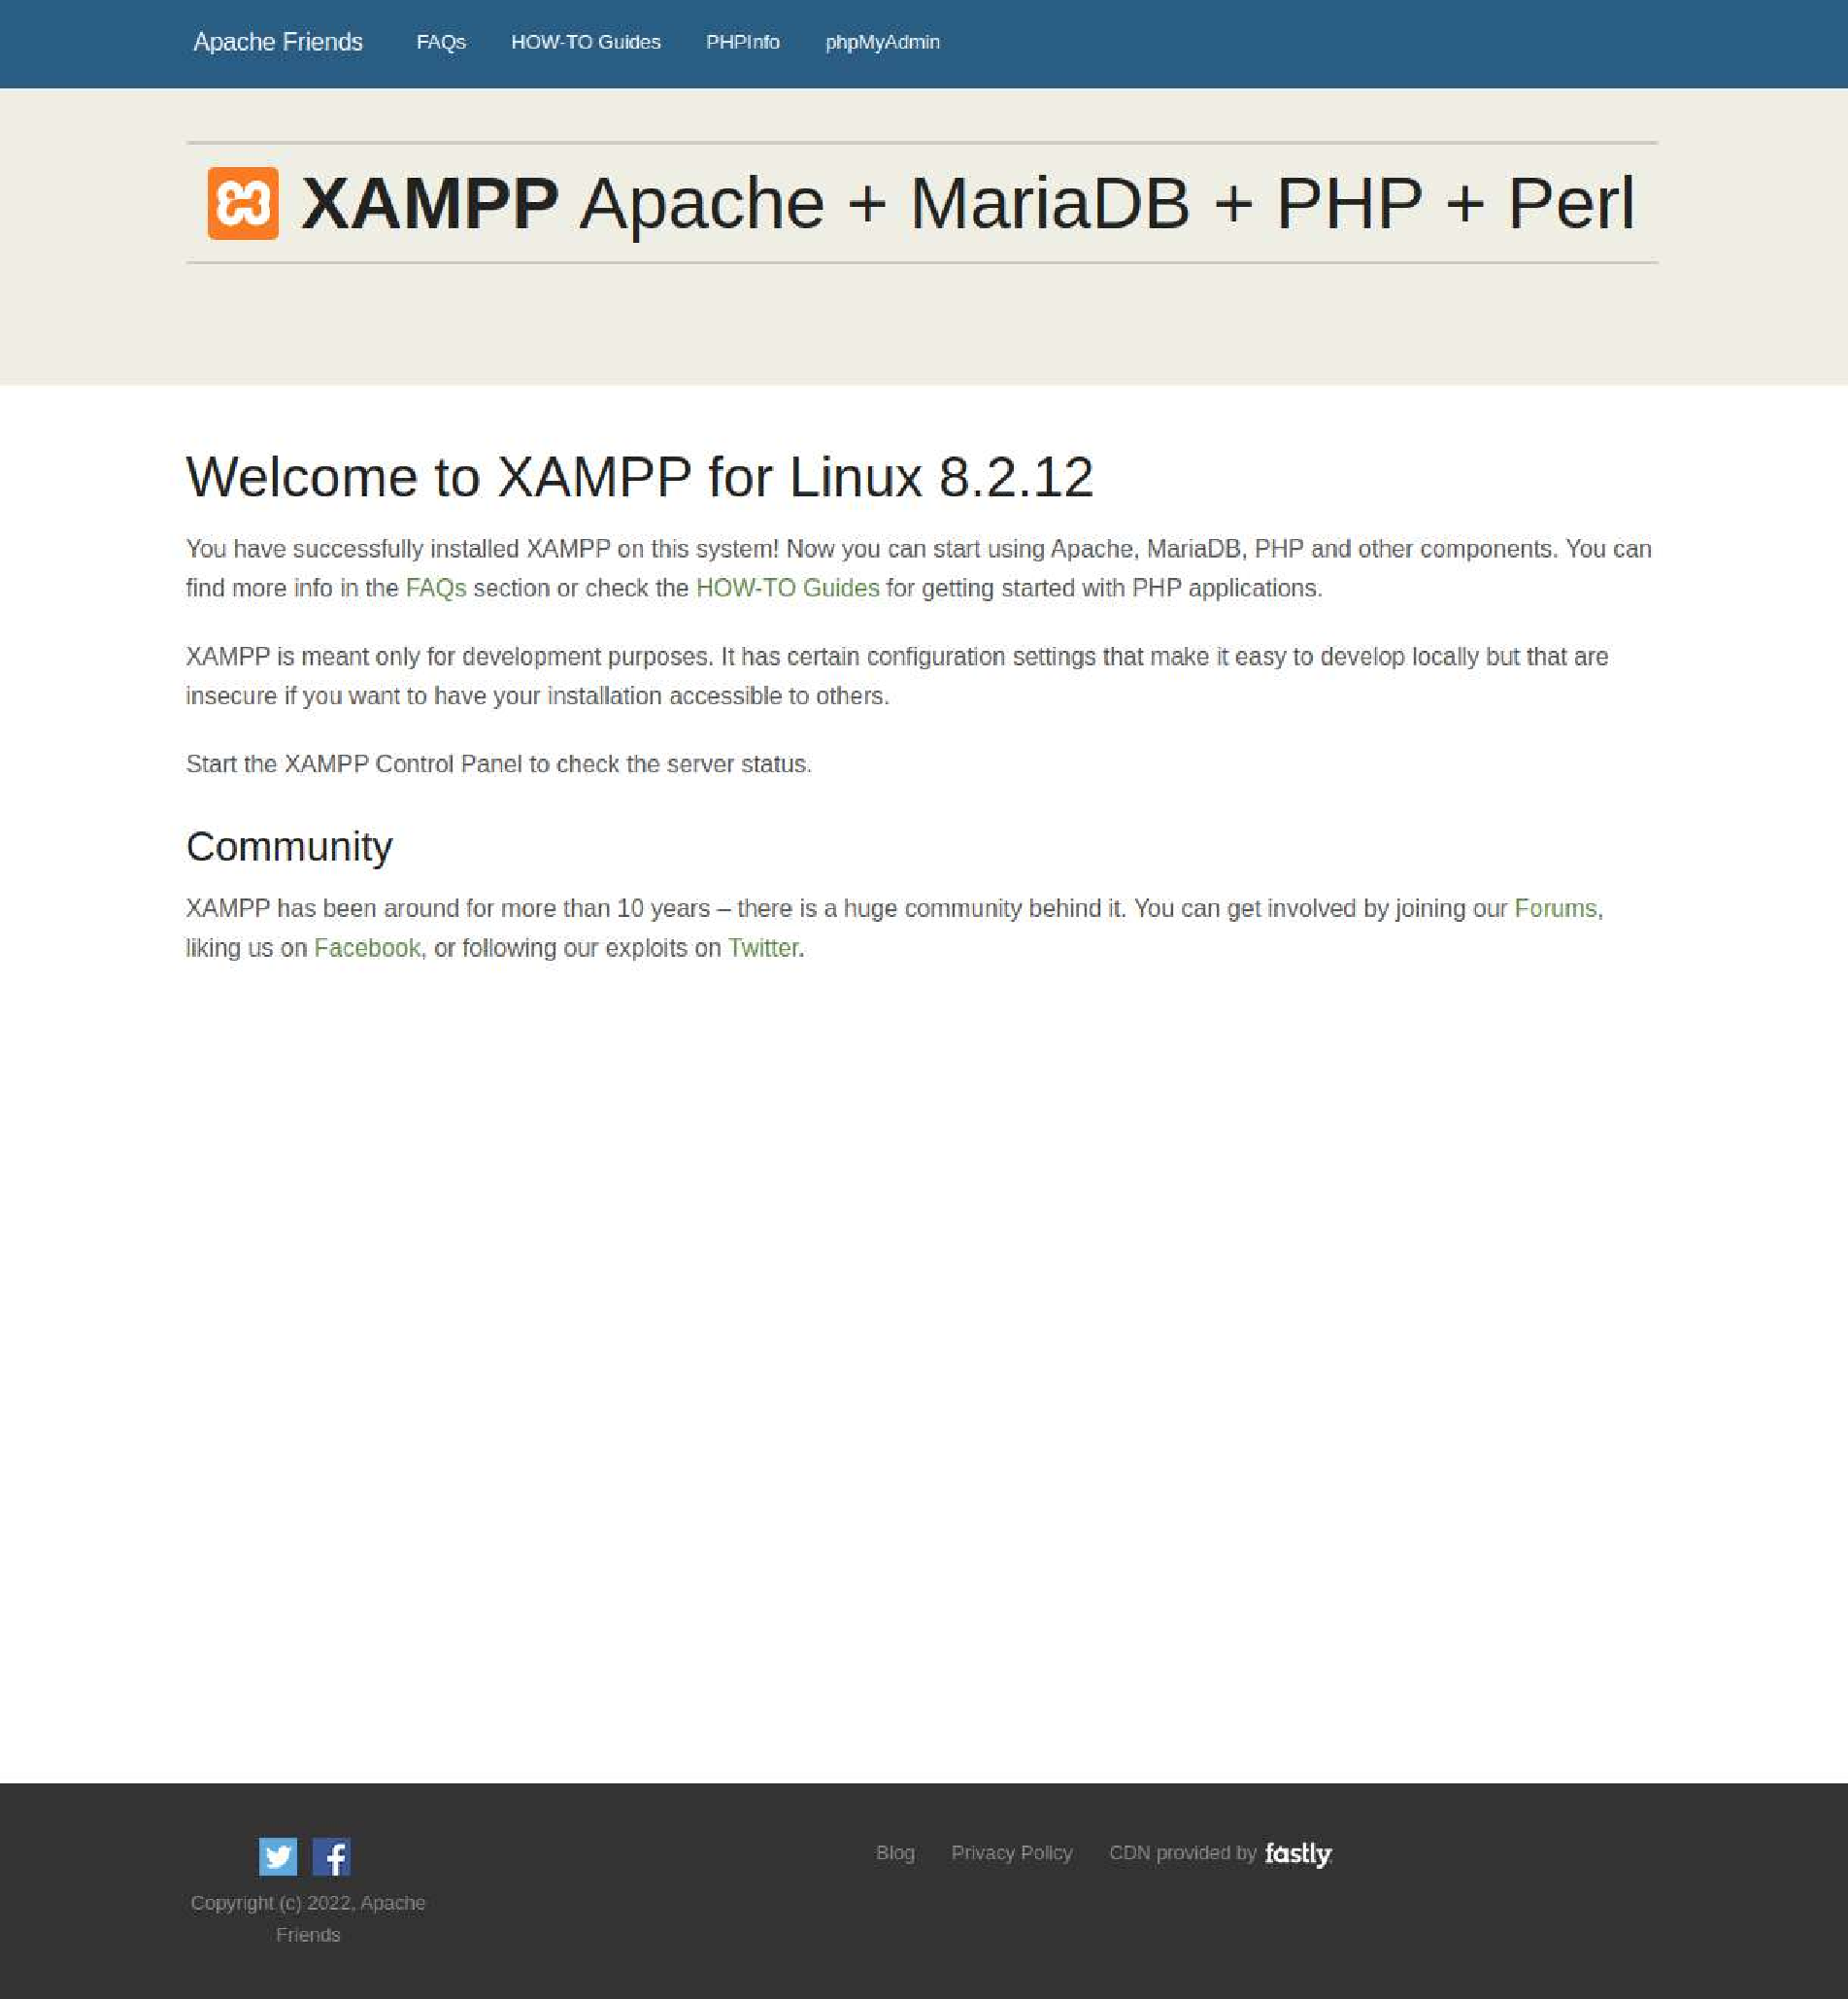
\includegraphics[width=0.9\linewidth]{figure/1.pdf}
  \caption{Welcome to XAMPP}
\end{figure}

\subsection*{実験Ⅱ:Webページ作成とデータベース構築}

本実験では,HTMLによるWebページの作成と,phpMyAdminを用いたデータベース(MariaDB)の作成・検索,およびPHPを用いたWebデータベースの構築を行った.

\subsubsection*{1. Webページの作成}

XAMPPのドキュメントルートに移動し,HTMLファイルを作成した.

\begin{lstlisting}[language=bash]
cd /opt/lampp/htdocs/
\end{lstlisting}

作成したファイル \texttt{sample.html} は以下の通りである.

\begin{lstlisting}[language=html]
<!DOCTYPE html>
<html>
<head>
<meta http-equiv="Content-Type" content="text/html; charset=utf-8"/>
<title>こんにちは</title>
</head>
<body>
<h1>見出し</h1>
<p>文章を書きましょう</p>
</body>
</html>
\end{lstlisting}

これをブラウザで \texttt{http://localhost/sample.html} にアクセスすることで表示を確認した.

次に,CSSによって文字色を赤く変更したスタイルを追加した.

\begin{lstlisting}[language=html]
<style>
 p {
   color: red;
 }
</style>
\end{lstlisting}

\begin{figure}[htbp]
  \centering
  
\includegraphics[width=0.9\linewidth]{figure/2.pdf}
  \caption{sample.html}
\end{figure}

\subsubsection*{2. データベースの作成・検索}

\texttt{phpMyAdmin}を用いて,データベース \texttt{maizuru} を作成し,以下の2つのテーブルを構築した.

\vspace{0.5zh}
\begin{itemize}
  \item \textbf{nameテーブル}:no, name(TEXT型)
  \item \textbf{birthplaceテーブル}:name, birthplace(TEXT型)
\end{itemize}

データを追加後,以下のSQL文でデータを検索・表示した.

\begin{lstlisting}[language=SQL]
SELECT * FROM name;
\end{lstlisting}

\begin{figure}[htbp]
  \centering
  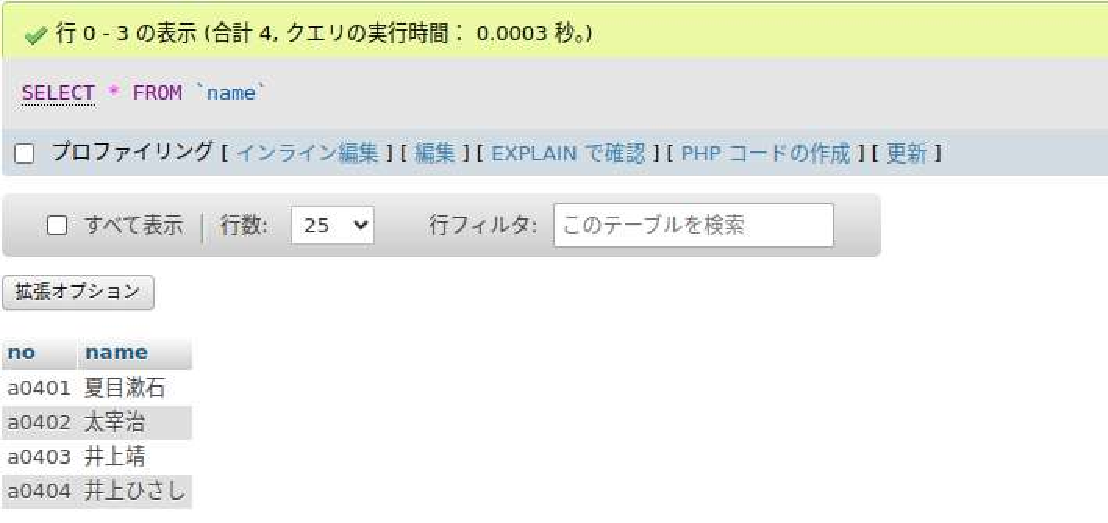
\includegraphics[width=0.9\linewidth]{figure/3.pdf}
  \caption{\texttt{maizuru} のnameテーブル}
\end{figure}

\begin{figure}[htbp]
  \centering
  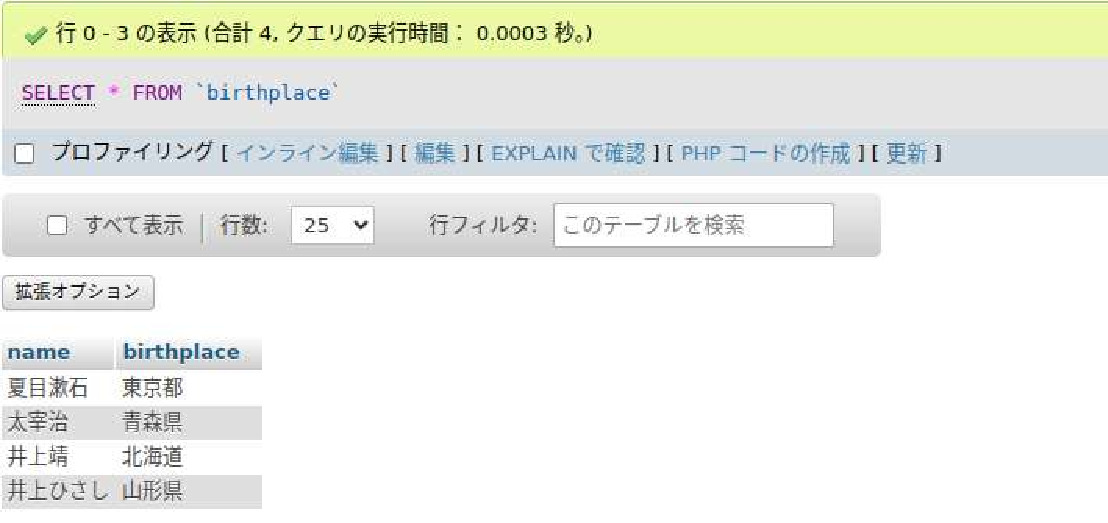
\includegraphics[width=0.9\linewidth]{figure/4.pdf}
  \caption{\texttt{maizuru} のbirthplaceテーブル}
\end{figure}

さらに,2つのテーブルを結合して,対応する生誕地を表示するクエリを実行した.

\begin{lstlisting}[language=SQL]
SELECT name.no, name.name, birthplace.birthplace 
FROM name 
INNER JOIN birthplace 
ON name.name = birthplace.name;
\end{lstlisting}

\subsubsection*{3. Webデータベースの構築(PHP)}

MariaDBのパスワードを設定するため,\texttt{--skip-grant-tables} モードで起動し,次のコマンドでパスワードを直接設定した.

\begin{lstlisting}[language=bash]
sudo /opt/lampp/sbin/mysqld --skip-grant-tables --skip-networking &
sudo /opt/lampp/bin/mysql -u root

UPDATE mysql.user 
SET authentication_string = PASSWORD('password') 
WHERE User = 'root' AND Host = 'localhost';
FLUSH PRIVILEGES;
sudo killall mysqld
sudo /opt/lampp/lampp start
\end{lstlisting}

その後,PHPを用いた接続確認とデータ表示のため,以下のファイルを配置した.

\textbf{connect.php}
\begin{lstlisting}[language=php]
    <html>
    <head>
    <meta http-equiv="Content-Type" content="text/html; charset=utf-8"/>
    <title>PHP TEST</title>
    </head>
    <body>
    
    <?php
    
    $link = mysqli_connect('localhost', 'root', 'password');
    if (!$link) {
        die('接続失敗です。'.mysql_error());
    }
    
    print('<p>接続に成功しました。</p>');
    
    $db_selected = mysqli_select_db($link,'maizuru');
    if (!$db_selected){
        die('データベース選択失敗です。'.mysql_error());
    }
    
    print('<p>データベースを選択しました。</p>');
    
    // MySQLに対する処理
    
    $close_flag = mysqli_close($link);
    
    if ($close_flag){
        print('<p>切断に成功しました。</p>');
    }
    
    ?>
    </body>
    </html>
\end{lstlisting}

\begin{figure}[htbp]
  \centering
  
\includegraphics[width=0.9\linewidth]{figure/6.pdf}
  \caption{connect.php}
\end{figure}

\textbf{select.php}
\begin{lstlisting}[language=php]
    <html>
    <head>
    <meta http-equiv="Content-Type" content="text/html; charset=utf-8"/>
    <title>PHP TEST</title>
    </head>
    <body>
    
    <?php
    
    $link = mysqli_connect('localhost', 'root', 'password');
    if (!$link) {
        die('接続失敗です。'.mysql_error());
    }
    
    print('<p>接続に成功しました。</p>');
    
    $db_selected = mysqli_select_db($link,'maizuru');
    if (!$db_selected){
        die('データベース選択失敗です。'.mysqli_error());
    }
    
    print('<p>データベースを選択しました。</p>');
    
    mysqli_set_charset($link,'utf8');
    
    $result = mysqli_query($link,'SELECT * FROM name');
    if (!$result) {
        die('クエリーが失敗しました。'.mysql_error());
    }
    
    while ($row = mysqli_fetch_assoc($result)) {
        print('<p>');
        print('id='.$row['no']);
        print(', name='.$row['name']);
        print('</p>');
    }
    
    $close_flag = mysqli_close($link);
    
    if ($close_flag){
        print('<p>切断に成功しました。</p>');
    }
    
    ?>
    </body>
    </html>
\end{lstlisting}
\begin{figure}[htbp]
  \centering
  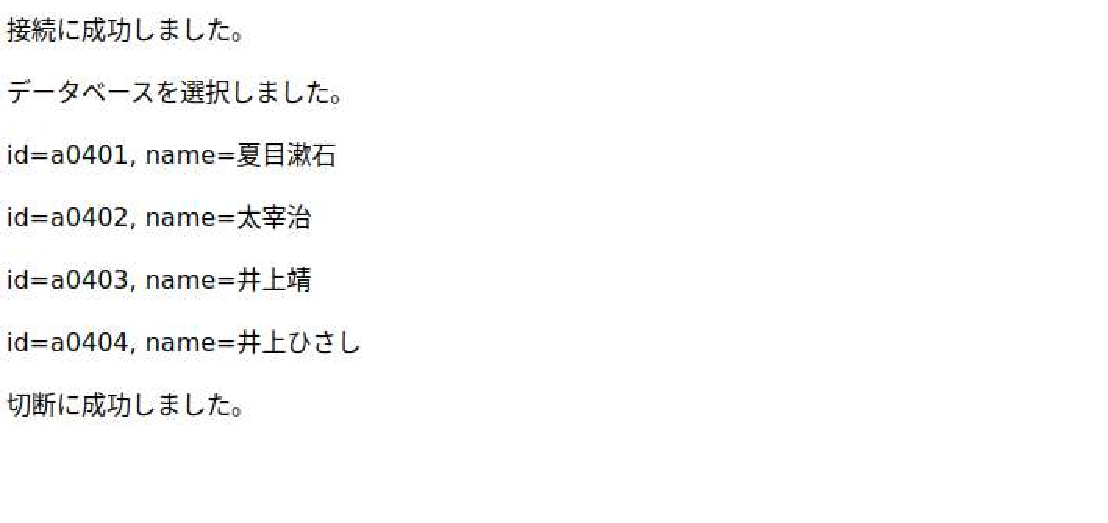
\includegraphics[width=0.9\linewidth]{figure/7.pdf}
  \caption{select.php}
\end{figure}

\textbf{select2.php}
\begin{lstlisting}[language=php]
    <html>
    <head>
    <meta http-equiv="Content-Type" content="text/html; charset=utf-8"/>
    <title>PHP TEST</title>
    </head>
    <body>
    
    <?php
    
    $link = mysqli_connect('localhost', 'root', 'password');
    if (!$link) {
        die('接続失敗です。'.mysql_error());
    }
    
    print('<p>接続に成功しました。</p>');
    
    $db_selected = mysqli_select_db($link,'maizuru');
    if (!$db_selected){
        die('データベース選択失敗です。'.mysql_error());
    }
    
    print('<p>データベースを選択しました。</p>');
    
    mysqli_set_charset($link,'utf8');
    
    $result = mysqli_query($link,'SELECT name.no, name.name, birthplace.birthplace FROM name inner join birthplace on name.name=birthplace.name');
    if (!$result) {
        die('クエリーが失敗しました。'.mysqli_error());
    }
    
    while ($row = mysqli_fetch_assoc($result)) {
        print('<p>');
        print('id='.$row['no']);
        print(', name='.$row['name']);
        print(', birthplace='.$row['birthplace']);
        print('</p>');
    }
    
    $close_flag = mysqli_close($link);
    
    if ($close_flag){
        print('<p>切断に成功しました。</p>');
    }
    
    ?>
    </body>
    </html>
\end{lstlisting}
\begin{figure}[htbp]
  \centering
  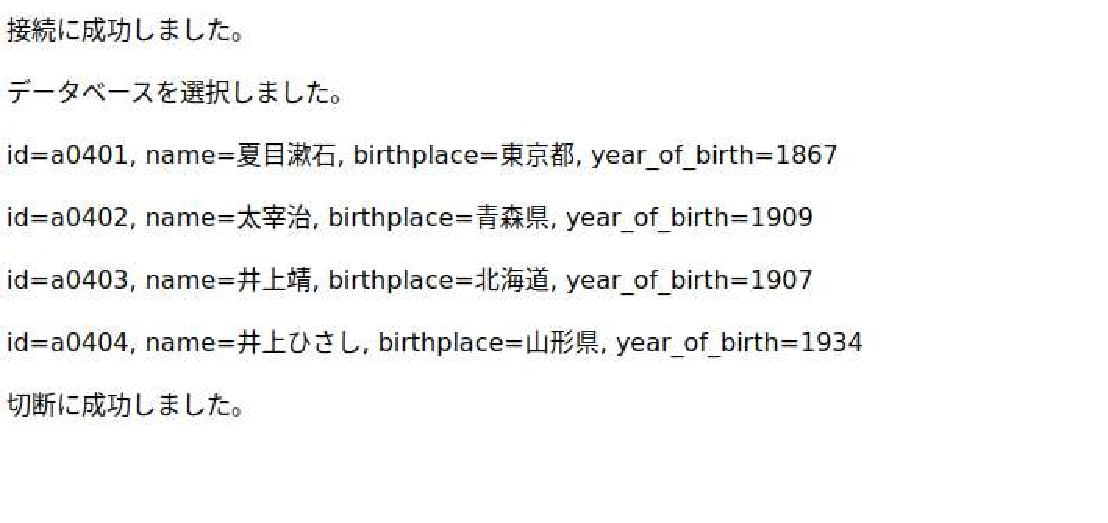
\includegraphics[width=0.9\linewidth]{figure/8.pdf}
  \caption{select2.php}
\end{figure}

\textbf{form\_name.html}(入力フォーム)

\begin{lstlisting}[language=html]
  <html>

  <head>
    <meta http-equiv="Content-Type" content="text/html; charset=utf-8" />
    <title>検索</title>
  </head>
  
  <body>
    <form action="regist.php" method="post">
      番号:<br />
      <input type="text" name="no" size="30" value="" /><br />
      名前:<br />
      <input type="text" name="name" size="30" value="" /><br />
      出身地:<br />
      <input type="text" name="birthplace" size="30" value="" /><br />
      生年:<br />
      <input type="text" name="year_of_birth" size="30" value="" /><br />
      <br />
      <input type="submit" value="登録する" />
    </form>
  </body>
  
  </html>
\end{lstlisting}
\begin{figure}[htbp]
  \centering
  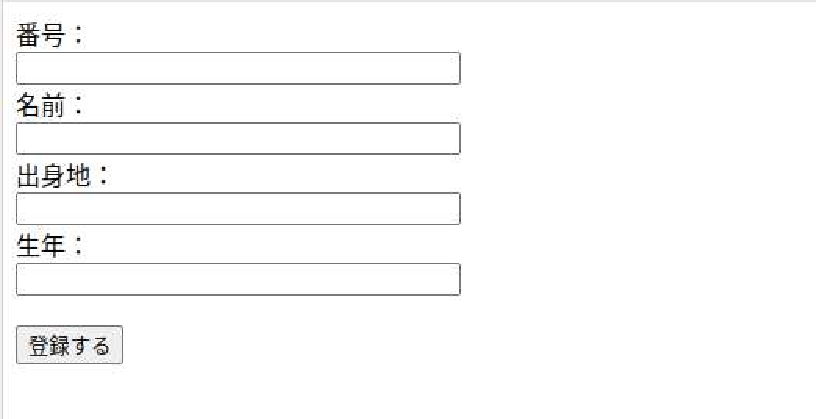
\includegraphics[width=0.9\linewidth]{figure/9.pdf}
  \caption{form\_name.html}
\end{figure}


これにより,Webフォームからデータベースへ動的に登録し,登録結果を確認する一連のWebデータベース操作が可能となった.

\subsection*{実験Ⅲ:Google Maps API を活用した Web データベースの構築}

本実験では,Google Maps API を活用して,データベースに登録された地理情報を地図上に可視化する Web アプリケーションを構築した.

\subsubsection*{1. データベースの作成}

phpMyAdmin にて,データベース \texttt{map} を新規作成し,以下の構成で \texttt{markers} テーブルを作成した.

\begin{lstlisting}[language=SQL]
CREATE TABLE `markers` ( 
  `id` INT NOT NULL AUTO_INCREMENT PRIMARY KEY, 
  `name` VARCHAR(60) NOT NULL, 
  `address` VARCHAR(80) NOT NULL, 
  `lat` FLOAT(10,6) NOT NULL, 
  `lng` FLOAT(10,6) NOT NULL, 
  `type` VARCHAR(30) NOT NULL 
) ENGINE = MYISAM;
\end{lstlisting}

初期データとして以下のようなレコードを登録した.

\begin{lstlisting}[language=SQL]
INSERT INTO `markers` (`name`, `address`, `lat`, `lng`, `type`)
VALUES ('Love.Fish', '580 Darling Street, Rozelle, NSW', -33.861034, 151.171936, 'restaurant');
\end{lstlisting}

\subsubsection*{2. データ出力用PHPスクリプト}

登録されたデータを XML 形式で出力するため,\texttt{toxml.php} を作成した.このスクリプトは,SQL クエリにより \texttt{markers} テーブルから全レコードを取得し,Google Maps JavaScript API が読み取れる形式の XML に変換して出力する.

\subsubsection*{3. Google Maps APIによる表示ページの構築}

\texttt{gis01.html},\texttt{gis02.html},\texttt{index.html} を作成し,Google Maps 上にマーカーとしてデータを描画した.

\paragraph*{gis01.html}
基本的な地図表示を行うページであり,以下のように初期表示位置とズームレベルを設定している:

\begin{lstlisting}[language=javascript]
map = new google.maps.Map(document.getElementById('map'), {
  center: {lat: -34.397, lng: 150.644},
  zoom: 8
});
\end{lstlisting}

\paragraph*{gis02.html}
\texttt{toxml.php} から取得した XML を解析し,地図上に各マーカーを配置する.

\paragraph*{index.html}
ユーザが地図上で検索できる UI を提供する.JavaScript(\texttt{script.js})により,検索ボックスやマーカーの追加が行われ,より直感的な操作が可能となる.

\subsubsection*{4. JavaScript によるマーカー描画(script.js)}

Google Maps API の \texttt{places} ライブラリと非同期通信(AJAX)を利用し,XML データを解析して地図上にマーカーを配置する処理は以下の通りである.

\begin{lstlisting}[language=javascript]
downloadUrl('toxml.php', function(data) {
  var xml = data.responseXML;
  var markers = xml.documentElement.getElementsByTagName('marker');
  ...
  var marker = new google.maps.Marker({
    map: map,
    position: point,
    label: icon.label
  });
\end{lstlisting}

マーカーをクリックすると,施設名と住所を表示する情報ウィンドウが開くように設定している.

